\documentclass[12pt]{article}
\usepackage[hmargin={.7in},vmargin={.7in}]{geometry}   
\geometry{letterpaper}       
%\geometry{landscape}          
%\usepackage[parfill]{parskip}
\usepackage{color,graphicx}
%\usepackage{covington}
%\usepackage{xyling}
\usepackage{setspace}
\usepackage{amsmath}
\usepackage{amssymb}
%\usepackage{graphicx,color}
%\usepackage{theorem}
%\usepackage{tabularx}
%\usepackage{subfig}
%\usepackage{vowel}
%\usepackage{mathrsfs}
\usepackage{varioref}
\usepackage{textcomp}
%\usepackage{avm}
\usepackage{textcomp}
\usepackage{mflogo}
\usepackage{wasysym}
%\usepackage{pstricks, pst-plot, pst-node, pst-tree, colortab}
%\usepackage{qtree}
 %\usepackage{tree-dvips}
 \usepackage{linguex}
%\usepackage{gb4e}
 \usepackage{multirow}
 %\usepackage[stable]{footmisc}
 \usepackage{pifont}
%\usepackage{todonotes}
%\usepackage{natbib}
\usepackage[normalem]{ulem}
\usepackage{wrapfig}

 %\setlength{\parskip}{.55ex plus 0.1ex}


\usepackage{fancyhdr} % This should be set AFTER setting up the page geometry
\pagestyle{plain} % options: empty , plain , fancy
\lhead{}\chead{}\rhead{}
\renewcommand{\headrulewidth}{.3pt}
\lfoot{}\cfoot{\thepage}\rfoot{}
%\renewcommand{\footrulewidth}{.3pt}
\newcommand{\txtp}{\textipa}
\renewcommand{\rm}{\textrm}
\newcommand{\sem}[1]{\mbox{$[\![$#1$]\!]$}}
\newcommand{\lam}{$\lambda$}
\newcommand{\lan}{$\langle$}
\newcommand{\ran}{$\rangle$}
\newcommand{\type}[1]{\ensuremath{\left \langle #1 \right \rangle }}
\newcommand{\defeq}{$\mathrel{\mathop:}=$ }
\renewcommand{\and}{$\wedge$ }


%\renewcommand{\Extopsep}{2pt}


\newcommand{\bex}{\begin{examples}}
\newcommand{\eex}{\end{examples}}

%bullet points
\newcommand{\bit}{\begin{itemize}}
\newcommand{\eit}{\end{itemize}}

%numbering, non sequential
\newcommand{\ben}{\begin{enumerate}}
\newcommand{\een}{\end{enumerate}}

\renewcommand{\abstractname}{The goal:}


%numbering, what you would use in a paper when you don't want the numbering to stop every time you end an example. 
%\newcommand{\bex}{\begin{enumerate}\setcounter{enumi}{\thesaveenumi}\item{}\begin{enumerate}}
%\newcommand{\eex}{\end{enumerate}\setcounter{saveenumi}{\theenumi}\end{enumerate}}

%%these are the brackets used for writing up semantic meanings 
%\newcommand{\lbr}{\textrm{\textlbrackdbl}}
%\newcommand{\rbr}{\textrm{\textrbrackdbl}}
%\renewcommand{\rm}{\textrm}

%this describes the numbering system (roman vs arabic numerals and so forth)
\renewcommand\theenumi {\alph{enumi}}
\renewcommand\theenumii {\alph{enumii}}
\renewcommand\labelenumi {\theenumi. }
\renewcommand\labelenumii {\theenumii.}
\labelformat{enumi}{(\theenumi)}
\labelformat{enumii}{(\theenumi\theenumii)}
\newcounter{saveenumi}

%\renewcommand{\labelitemi}{\textbf{---}}
%\renewcommand{\labelitemii}{\textbf{$\cdot$}}

%\linespread{1.5}

%\qtreecenterfalse

%\linespread{1}

\begin{document}

\begin{center}\textbf{Property subjectivity predicts adjective ordering preferences}
\end{center}
	
	\vspace{-15pt}
	
Cross-linguistically stable preferences for adjective ordering have been widely documented, yet the factors that determine these preferences are still poorly understood. Our approach to the investigation of adjective ordering preferences synthesizes strategies from the \emph{psychological approach}, probing the principles that underlie these preferences \cite{sweet1898,ziff1960,martin1969determinants,martin1969competence,martin1970,kemmereretal2009}, and from the \emph{grammatical approach}, using descriptive semantic classes of adjective to structure and inform our hypotheses \cite{dixon1982,sproatshih1991,cinque1994,scott2002}. 

\textbf{Exp.~1 (corpus study).} For 26 adjectives from seven different classes (size, quality, age, texture, shape, color, material; see Table 1 for the full list of adjectives), we extracted all cases of phrases with either two or three adjectives (e.g., ``a good green color'' or ``some big new red cloaks'') from the Switchboard and the British National Corpus (for a total of 39,199 cases). For each adjective, we  computed its mean distance from the modified noun. Means by adjective class are shown in Fig.~1 (corpus). Pairwise Bonferroni-corrected comparisons between classes on the mean distance-from-noun scores yields the following ordering preferences, which closely track the previous reports in the literature \cite{sproatshih1991,dixon1982}:
%\vspace{-13pt}
\emph{size} $\geq$ \emph{quality} $>$  \emph{age} $>$  \emph{texture} $>$  \emph{shape} $>$  \emph{color} $>$  \emph{material}. %\label{inferred-order-preferences}$$

%\vspace{-13pt}

\textbf{Exp.~2 (n=50)} used behavioral measures to closely replicate these inferred ordering preferences. We elicited naturalness judgments on adjective-adjective-noun object descriptions, permuting the relative order of the adjectives. We used the same adjectives from the corpus experiment, paired at random with a set of ten nouns describing either food or furniture (see Table 1 for the full list of words).
Participants indicated which ordering of an adjective-adjective-noun object description sounded more ``natural,'' using a sliding scale with endpoints labeled with the competing object descriptions (e.g., ``the big red apple'' vs.\ ``the red big apple''). On the basis of these naturalness ratings, we computed for each adjective-adjective pairing its preferred, canonical order (i.e., the order with the highest naturalness rating). We then determined how often an adjective from a given semantic class occurred first in a preferred adjective-adjective-noun configuration; Fig.~1 (preference) plots these mean distance-from-noun scores, where a value of 1 signals that a class's adjectives always occur first in preferred adjective-adjective-noun orderings. 

Having established the robustness of ordering preferences both in production (Exp.~1) and in comprehension (Exp.~2), we then shifted focus to the source of these preferences. While researchers disagree about the details, psychological explorations of ordering preferences have converged on the idea that aspects of  adjectives' meaning (e.g., specificity, context-sensitivity, reliance on comparison) determine their relative order \cite{sweet1898,ziff1960,martin1969determinants,martin1969competence,martin1970,kemmereretal2009}. % On the basis of the preferred orderings we observed both in the corpus and in our behavioral experiment, 
We distilled the proposals that precede us into a single feature: the subjectivity of the property named. In each of the observed preferred orderings, intuition suggests that less subjective adjectives appear closer to the modified noun. 

\textbf{Exp.~3 (n=45)} tested this subjectivity hypothesis  by estimating the subjectivity of adjectives (and the classes to which they belong) using a faultless disagreement measure. Participants evaluated the potential for faultless disagreement between two differing descriptions of an object. For example, an experimental trial would have Mary assert ``that apple is old,'' then have Bob counter with ``that apple is not old.'' 
To the extent that both Mary and Bob can be right in their descriptions of the apple, ``old'' admits that degree of faultless disagreement. 
Thus, the extent to which two people can disagree about a description without one necessarily being wrong determines the subjectivity of that description. 
We validated the faultless disagreement measure in a separate paradigm (n=30), in which participants rated the ``subjectivity'' of object descriptions directly; the results of these two methods were highly correlated ($r^{2} = 0.89$), suggesting that faultless disagreement is a good proxy for subjectivity.
Fig.~1 (subjectivity) plots mean faultless disagreement ratings for adjectives and their respective classes. Based on pairwise comparisons of these aggregate scores, we inferred the following adjective class subjectivity ranking: 	\emph{quality} $\geq$ \emph{size} $>$ \emph{texture} $\geq$ \emph{age} $>$ \emph{color}
	$\geq shape \geq material$.
This ranking closely tracks the inferred order preferences from Exps.~1 and 2.
\begin{wrapfigure}[50]{r}{.42\linewidth}
	%\vspace{-30pt}
	Table 1: The adjectives and their classes tested in all experiments, and the nouns and their classes tested in the behavioral experiments. \\
	{\footnotesize \begin{tabular}{llll}
		\textbf{adjective}	&	\textbf{class}	&	\textbf{adjective}	&	\textbf{class}	\\ \hline
		old	&	age	&	good	&	quality	\\
		new	&	age	&	bad	&	quality	\\
		rotten	&	age	&	round	&	shape	\\
		fresh	&	age	&	square	&	shape	\\
		red	&	color	&	big	&	size	\\
		yellow	&	color	&	small	&	size	\\
		green	&	color	&	huge	&	size	\\
		blue	&	color	&	tiny	&	size	\\
		purple	&	color	&	short	&	size	\\
		brown	&	color	&	long	&	size	\\
		wooden	&	material	&	smooth	&	texture	\\
		plastic	&	material	&	hard	&	texture	\\
		metal	&	material	&	soft	&	texture	\\
		\textbf{noun}	&	\textbf{class}	&	\textbf{noun}	&	\textbf{class}	\\ \hline
		apple	&	food	&	chair	&	furniture	\\
		banana	&	food	&	couch	&	furniture	\\
		carrot	&	food	&	fan	&	furniture	\\
		cheese	&	food	&	TV	&	furniture	\\
		tomato	&	food	&	desk	&	furniture	
	\end{tabular}}
	\vspace{-10pt}
	\begin{center}
		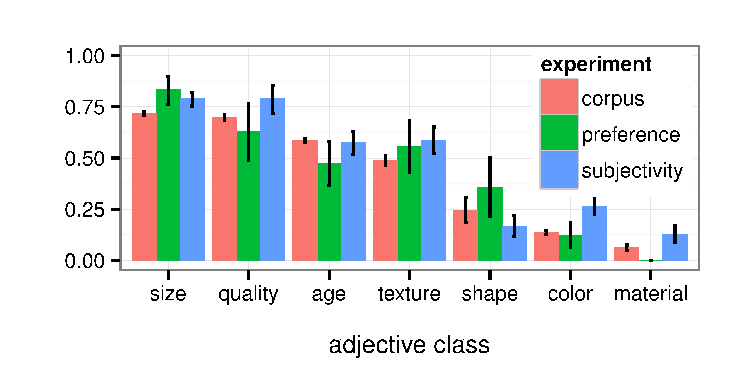
\includegraphics[width=\linewidth]{plots/expt_results.eps}
	\end{center}
	\vspace{-15pt}
	Fig.~1: Mean distance from noun (corpus), mean preferred distance from noun  (preference), and mean faultless disagreement scores (subjectivity) for adjectives by their semantic class.
	\vspace{-10pt}
	\begin{center}
		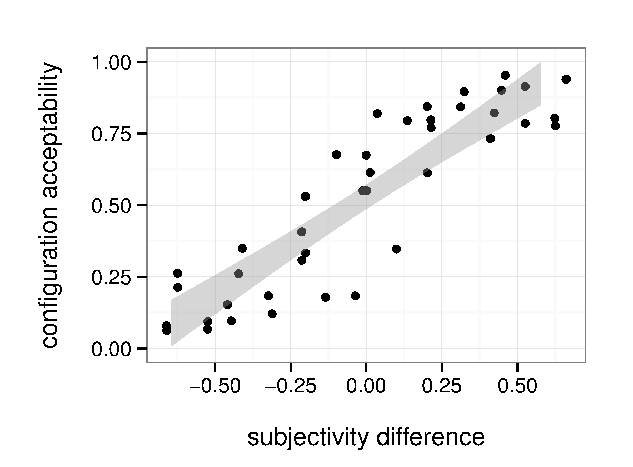
\includegraphics[width=.9\linewidth]{plots/comparison2.eps}
	\end{center}
	\vspace{-10pt}
	Fig.~2: Class-level order preferences plotted against faultless disagreement difference scores.
\end{wrapfigure}
%\vspace{0pt}
%\vspace{-13pt}
%\begin{center}
%	\vspace{-14pt}
%	$quality \geq size > texture \geq age > color$\\
%	$\geq shape \geq material$
%\end{center}
%\vspace{-11pt}
\vspace{-15pt}

To evaluate the power of subjectivity in predicting adjective order, we compared naturalness ratings (Exp.~2) to faultless disagreement scores (Exp.~3). We  computed a subjectivity difference score for each class configuration (i.e., an ordered pairing of two adjective classes, \textsc{class1}-\textsc{class2}) by subtracting the mean faultless disagreement score for \textsc{class1} from the mean faultless disagreement score for \textsc{class2}. Higher difference scores indicate that the adjective class closer to the noun is less subjective than the class farther away. Fig.~2 plots naturalness ratings  against these faultless disagreement difference scores; the two measures are highly correlated ($r^2$ = 0.81), strongly supporting the hypothesis that less subjective adjectives occur more closely to the noun.

Adjective ordering preferences have received considerable attention throughout the history of generative grammar and cognitive psychology, owing to its remarkable stability within and across languages. Something so robust, the reasoning goes, must evidence a deep principle of the cognitive architecture that shapes language. Yet while descriptions of the phenomenon abound, an explanation continues to prove elusive. Our findings serve to narrow the space of possible explanations: rather than representing these preferences as a fully specified ranking according to semantic classes or syntactic projections, our results demonstrate that ordering preferences more likely emerge from a desire to place more informative, less subjective content closer to the substantive head of a nominal construction (i.e., closer to the modified noun).

\vspace{10pt}
\noindent
\footnotesize
	\textbf{References:} 
	[1]  Sweet (1898), {\em A New English Grammar};
	[2]  Ziff (1960), {\em Semantic Analysis};
	[3]  Martin (1969), {\em Semantic Determinants of Preferred Adjective Order}, J.~of Verbal Learning and Verbal Behavior, 8, 697--704;
	[4]  Martin (1969), {\em Some Competence-Process Relationships in Noun Phrases with Prenominal and Postnominal Adjectives}, J.~of Verbal Learning and Verbal Behavior, 8, 471--480;
	[5]  Martin (1970), {\em Adjective Order and Juncture}, J.~of Verbal Learning and Verbal Behavior, 9, 379--383;
	[6] Kemmerer, Tranel \& Zdansczyk (2009). {\em Knowledge of the semantic constraints on adjective order can be selectively impaired}, J.~of Neurolinguistics, 22, 91--108;
	[7]  Dixon (1982), {\em Where have all the adjectives gone?, and other essays in semantics and syntax};
	[8]  Sproat \& Shih (1991). {\em The cross-linguistic distribution of adjective ordering restrictions}, Interdisciplinary approaches to language: Essays in honor of S.-Y.~Kuroda (1991), 565--593;
	[9]  Cinque (1994), {\em On the evidence for patial N-movement in the Romance DP}, Paths towards Universal Grammar. Studies in honor of Richard S.~Kayne, 85--110;
	[10]  Scott (2002), {\em Stacked adjectival modification and the structure of nominal phrases}, The Cartography of Syntactic Structures, 91--120.
	
	
\newpage

\begin{thebibliography}{10}
	
	\bibitem{sweet1898}
	H.~Sweet, {\em A New English Grammar} (1898).
	
	\bibitem{ziff1960}
	P.~Ziff, {\em Semantic Analysis} (1960).
	
	\bibitem{martin1969determinants}
	J.~E.~Martin, {\em Semantic Determinants of Preferred Adjective Order}, Journal of Verbal Learning and Verbal Behavior, 8 (1969), pp.~697--704. 
	
	\bibitem{martin1969competence}
	J.~E.~Martin, {\em Some Competence-Process Relationships in Noun Phrases with Prenominal and Postnominal Adjectives}, Journal of Verbal Learning and Verbal Behavior, 8 (1969), pp.~471--480. 
	
	\bibitem{martin1970}
	J.~E.~Martin, {\em Adjective Order and Juncture}, Journal of Verbal Learning and Verbal Behavior, 9 (1970), pp.~379--383. 

	\bibitem{kemmereretal2009}
	kemmerer
	
	\bibitem{dixon1982}	
	R.~M.W.~Dixon, {\em Where have all the adjectives gone?, and other essays in semantics and syntax} (1982).

	\bibitem{sproatshih1991}
	R.~Sproat and C.~Shih, 1991. {\em The cross-linguistic distribution of adjective ordering restrictions}, Interdisciplinary approaches to language: Essays in honor of S.-Y.~Kuroda (1991), pp.~565--593.
	
	\bibitem{cinque1994}
	G.~Cinque, {\em On the evidence for patial N-movement in the Romance DP}, Paths towards Universal Grammar. Studies in honor of Richard S.~Kayne (1994), pp.~85--110.
	
	\bibitem{scott2002}
	G.-J.~Scott, {\em Stacked adjectival modification and the structure of nominal phrases}, The Cartography of Syntactic Structures (2002), pp.~91--120.
\end{thebibliography}


%\bibliographystyle{chicago}
%\bibliography{greg.bib}




\end{document}






\noindent
\begin{minipage}[t]{.48\linewidth}
	\vspace{0pt}
	\begin{center}
		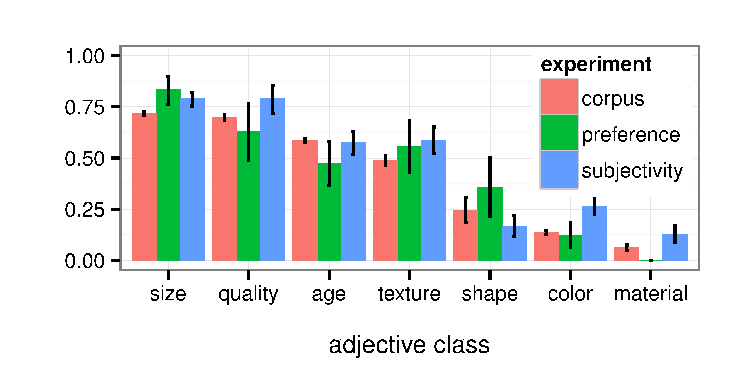
\includegraphics[width=\linewidth]{plots/expt_results.eps}
	\end{center}
	\vspace{-15pt}
	Fig.~1 (corpus results): Mean distance from noun by adjective class for cases with at least two modifying adjectives.
	Fig.~2 (Expt.~1 results): Mean preferred distance from noun for each adjective class.
	Fig.~3 (Expt.~2 results): Mean faultless disagreement scores for adjectives by class.
\end{minipage} \hfill
\begin{minipage}[t]{.46\linewidth}
	\vspace{0pt}	
	\begin{center}
		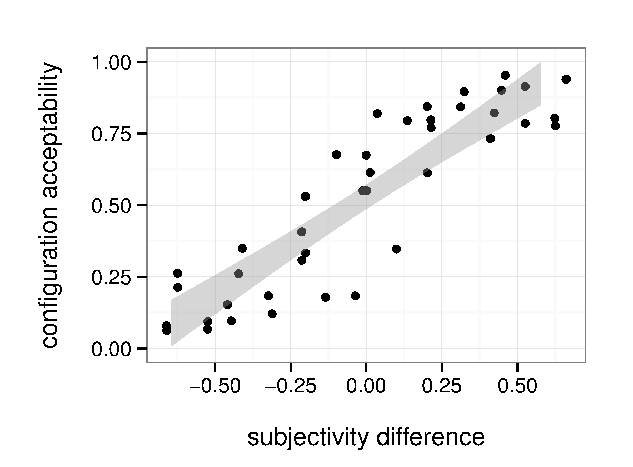
\includegraphics[width=\linewidth]{plots/comparison2.eps}
	\end{center}
	Fig.~4: Class-level order preferences plotted against difference in faultless disagreement between A1 and A2 (values greater than 0 indicate that the more subjective adjective class occurs farther from the noun).
\end{minipage}